% !TEX root = ../gnss_interference_resistant_thesis.tex
\documentclass[main.tex]{subfiles}

\begin{document}

\subsection{GPS sistema}

GPS (angl. Global Positioning system) yra palydovais paremta navigacinė
sistema, priklausanti Jungtinėms Amerikos Valstijoms. Ši sistema yra viena
iš kelių globalių navigacinių (GNSS) sistemų. Naudojantis GPS sistema,
galima nustatyti vartotojo buvimo vietą (ilgumą, platumą, aukštį), bei
galima tiksliai susinchronizuoti laiką. Šiuo metu yra teikiamos dvi GPS paslaugos:

\begin{itemize}
    \item Tikslaus pozicionavimo paslauga (PPS)\cite{pps_standard} skirta kariniam naudojimui
    \item Standartinė pozicionavimo paslauga (SPS)\cite{sps_standard}
    atvira civiliniam naudojimui.
\end{itemize}

\noindent Šiame darbe bus nagrinėjami tik SPS signalai.

\subsubsection{Pozicijos ir laiko nustatymas}

Kad imtuvas galėtų nusistatyti savo poziciją, jam reikia priimti signalą bent
iš 4 palydovų. GPS signalas sudarytas taip, kad būtų galima išmatuoti atstumą iki
kiekvieno palydovo, signale yra užkoduotas išsiuntimo laikas, todėl priėmus
signalą iš palydovo, žinant tikslų imtuvo laiką ($t_{imtuvo}$), sklidimo greitį ($c$),
išsiuntimo laiką ($t_{siustuvo}$), galima išmatuoti signalo keliavimo trukmę ir suskaičiuoti
atstumą ($l$) iki palydovo:

\begin{equation}
    l = c (t_{imtuvo} - t_{siustuvo}).
\end{equation}

\subsubsection{GPS signalas}\label{sec:gps_signal}

Visi GPS palydovai siunčia apskritimiškai poliarizuotą signalą, trijose skirtingose
dažnių juostose: L1 - $1575,42\ \mathrm{MHz}$, L2 - $1227,60\ \mathrm{MHz}$ ir
L5 - $1176,45\ \mathrm{MHz}$\cite{sps_standard}. Šiame darbe naudojimui pasirinktas
L1 signalas, kadangi jis yra palaikomas visų GPS palydovų, bei supaprastina imtuvų
konstrukciją, kadangi nereikia priimti signalų skirtingose dažnių juostose, todėl toliau
bus nagrinėjamas tik L1 signalas.

L1 signalo nešlys susideda iš dviejų komponentų kurių fazė skiriasi $90\degree$.
Kiekvienas nešlio komponentas yra faziškai moduliuojamas atskirų skaitmeninių signalų.
Pirmasis nešlio komponentas yra koduojamas P(Y) kodo ir LNAV duomenų (50 bitų/s) suma.
P(Y) kodas yra skirtas tikslios pozicijos nustatymui, ir šiuo metu jis yra užkoduotas
kariniam naudojimui.
LNAV duomenys yra skirti perduoti imtuvui tam tikrus GPS sistemos parametrus, tokius
kaip orbitos duomenis, laikrodžio korekcijos ir kita.
Antroji nešlio dalis yra moduliuojama C/A (netikslaus sekimo) kodu ir tais pačiai LNAV
duomenimis. C/A kodas yra 1023 "čirpų" ilgio ir jo dažnis yra $1.023\ \mathrm{MHz}$.
C/A kodas yra naudojamas signalo sklidimo trukmei matuoti. GPS signalas gali būti
aprašomas šia lygtimi:

\begin{equation}
    x_{IN}[k] = A(t) \widetilde{s_T}(t-\tau(t))e^{j(2\pi f_D(t)t+\phi(t))} |_{t=kT_s} + n(t) |_{t=kT_s},
    \label{eq:gps_signal}
\end{equation}

\noindent čia $x_{IN}$ priimamas signalas, $A(t)$ - signalo amplitudė, $\widetilde{s_T}$
- kompleksinis GPS signalas, $\tau(t)$ - kodo vėlinimas, $f_D(t)$ - Doplerio dažnis,
$\phi(t)$ - nešlio fazė, $n(t)$ - triukšmai, $T_s$ - diskretizavimo dažnis imtuve.

\begin{figure}[h]
    \begin{centering}
    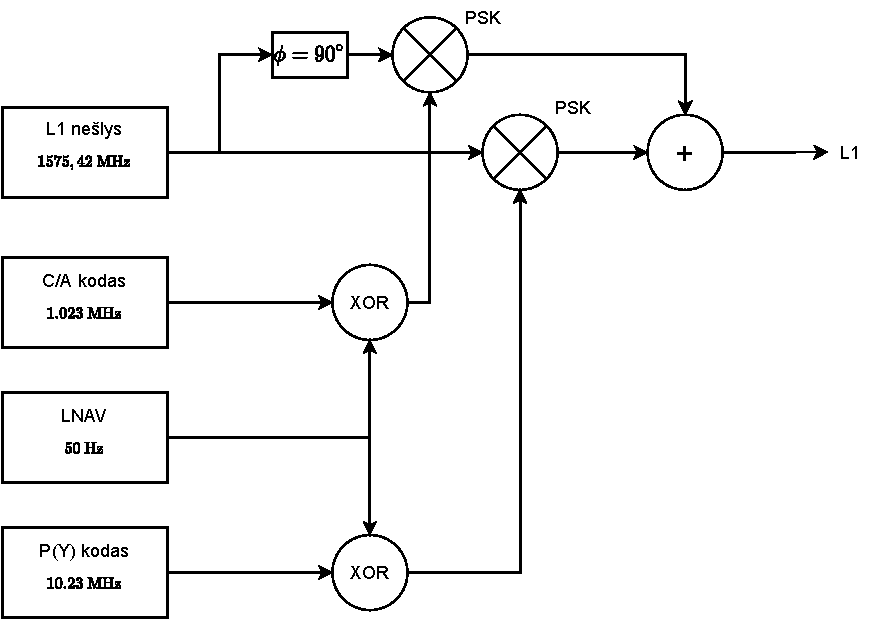
\includegraphics[scale=0.85]{drawings/l1_signal}
    \par\end{centering}
    \protect\caption{\label{fig:l1_signal}L1 signalo moduliatoriaus schema. Adaptuota iš \cite{Sadeghi2008TimeSS}.}
\end{figure}

Kadangi visi palydovai transliuoja tuo pačiu dažniu, C/A kodas pasirenkamas toks,
kad jis būtų pseudo-atsitiktinis kodas (PRN), kiekvienam palydovui yra suteikta unikali seka.
Svarbiausia PRN savybė - autokoreliacijos rezultato maksimumas yra tik
ties 0 tašku \cite{OCHIN202121_chapter2}.

Imtuvai ieškodami palydovo signalo, susigeneruoja ieškomo palydovo unikalią C/A signalo
kopiją ir atlieka koreliaciją tarp lokaliai sugeneruoto signalo ir priimto.
Iš gauto koreliacijos rezultato galima nustatyti gauto C/A signalo užlaikymą.

\subsubsection {GPS paklaidos}

Atliekami GPS signalo matavimai yra veikiami skirtingų tipų atsitiktinių ir sistematinių
paklaidų. Paklaidas galima suskirstyti į kelias pagrindines kategorijas \cite{KUMAR20213_chapter1}:

\begin{itemize}
    \item Palydovo ir imtuvo laikrodžio paklaidos
    \item Atspindžių paklaidos
    \item Atmosferinės paklaidos
    \item Orbitos paklaidos
\end{itemize}

Palydovuose naudojami atominiai laikrodžiai yra labai tikslūs, tačiau visi vien atsiranda paklaidos.
Tipinė palydovo laikrodžio paklaida yra $8-17\ \mathrm{ns}$ per dieną. Tokios paklaidos
gali būti eliminuotos priimant signalą iš kelių palydovų. Dėl laikrodžio netikslumų atsiranda
pozicijos paklaidos iki kelių metrų \cite{KUMAR20213_chapter1}.

GPS signalų sąveika su aplinka, pastatais, reljefu, sukelia atspindžių paklaidas. Kadangi
atsispindėjęs signalas nukeliauja didesnį atstumą, naudojantis tokiu signalu nebeįmanoma
tiksliai nustatyti atstumo iki palydovo, dėl to mažėja galutinės pozicijos tikslumas.

Atmosferinės paklaidos atsiranda dėl radijo bangų sklidimo parametrų kitimo atmosferoje ir
jonosferoje, kadangi parametrai pastoviai kinta laike, dėl besikeičiančių atmosferos/jonosferos
sąlygų. Dėl šių veiksnių atsiradusios paklaidos yra didžiausios lyginant su kitomis.
Šių trikdžių šalinimas įmanomas pasinaudojant korekcijomis iš antžeminių stočių, taip
pat galima priiminėti L1 ir L5 signalus. Kadangi šie signalai veikia skirtinguose
dažnių ruožuose, atmosferos reiškiniai juos veikia skirtingai, o kadangi
dažninės priklausomybės yra detaliai ištyrinėtos, todėl galima pašalinti
paklaidas išmatavus sklidimo trukmės skirtumus tarp L1 ir L5 signalo.

Kadangi orbitoje esantys palydovai yra veikiami nenuspėjamų jėgų, bėgant laikui jų orbitos
po truputį keičiasi. Norint pašalinti šias paklaidas, visi palydovai transliuoja savo
orbitos duomenis ir juos atnaujina kas 4 valandas \cite{sps_standard}. Palydovų orbitas
matuoja antžeminės GPS sistemos valdymo stotys, kurios perduoda šiuos duomenis
į palydovus, kad šie galėtų juos išsiųsti imtuvams per LNAV žinutes.

\end{document}
